\documentclass{article}
\usepackage[utf8]{inputenc}
\usepackage[spanish]{babel}
\usepackage{graphicx}
\usepackage{geometry}
\usepackage{enumerate}
\usepackage{titlesec}
\usepackage{float}
\usepackage{listings}
\usepackage{xcolor}
\usepackage{amsmath}
\usepackage{matlab-prettifier}
\usepackage{amssymb}
\usepackage{tabularx}

\geometry{letterpaper, margin = 1.5cm}

\newcommand{\codefontsize}{\fontsize{10}{11}}
\lstset{
	style = Matlab-editor,
	basicstyle = \codefontsize\ttfamily,
	mlshowsectionrules = true,
	upquote = true,
	tabsize = 4,
	captionpos = b,
	breaklines = true,
	breakatwhitespace = true,
	frame = single,
}

%Datos de la Portada
\title{Introducción a la Programación \ Practica 9}
\author{Medina Martinez Jonathan Jason \ 2023640061}
\date{06 de junio del 2023}

\begin{document}
	
	\fontsize{12}{16}\selectfont
	
	\begin{figure}[t]
		
		
\includegraphics[width=2.5 cm]{Logo1.jpeg}
		\hfill
		
\includegraphics[width=3 cm]{Logo2.png}
		
	\end{figure}
	
	\maketitle
	\newpage
	
	\tableofcontents
	\newpage
	
	\section{Objetivo}
	
	Implementar funciones para la captura de imágenes, utilizando un lenguaje de programación científico.
	
	\section{Introducción}
	
	La captura de imágenes mediante un periférico, como una cámara de video, se ha vuelto una tarea común y necesaria en diversas aplicaciones. En esta práctica, se busca implementar funciones para la captura de imágenes utilizando un lenguaje de programación científico. El objetivo principal es desarrollar un programa en MATLAB que permita abrir la cámara de video de un dispositivo, mostrar el video en tiempo real, capturar fotografías y visualizar el video en escala de grises. Para lograrlo, se utilizarán los paquetes de soporte de MATLAB para cámaras web USB y la interfaz genérica de video de Image Acquisition Toolbox.
	
	\newpage
	
	\section{Desarrollo}
	
	Escriba un programa que permita abrir la cámara de video de su dispositivo. Este programa deberá funcionar en MATLAB instalado y MATLAB Online. Para esto, deberá instalar los toolbox \textit{MATLAB Support Package for USB Webcams} y \textit{Image Acquisition Toolbox Support Package for OS Generic Video Interface}.
	
	El programa deberá:
	
	\begin{itemize}
		\item Mostrar el video de la cámara.
		\item Permitir tomar una fotografía.
		\item Permitir mostrar el video de la cámara en escala de grises.
	\end{itemize}
	
	\newpage
	
	\subsubsection{CAMARA.m}
	
	\begin{lstlisting}
		
	clc,clear;
	
	camara = webcam('Integrated Camera');
	
	preview(camara);
	
	imagen = snapshot(camara);
	imagen2 = snapshot(camara);
	imagenB = rgb2gray(imagen2);
	
	imshow(imagen);
	
	figure
	imshow(imagenB);
	
	closePreview(camara);
	clc,clear;
	
	\end{lstlisting}
	
	\newpage
	
	\subsubsection{Ejecución}
	
	\begin{figure*}[h]
		\centering
		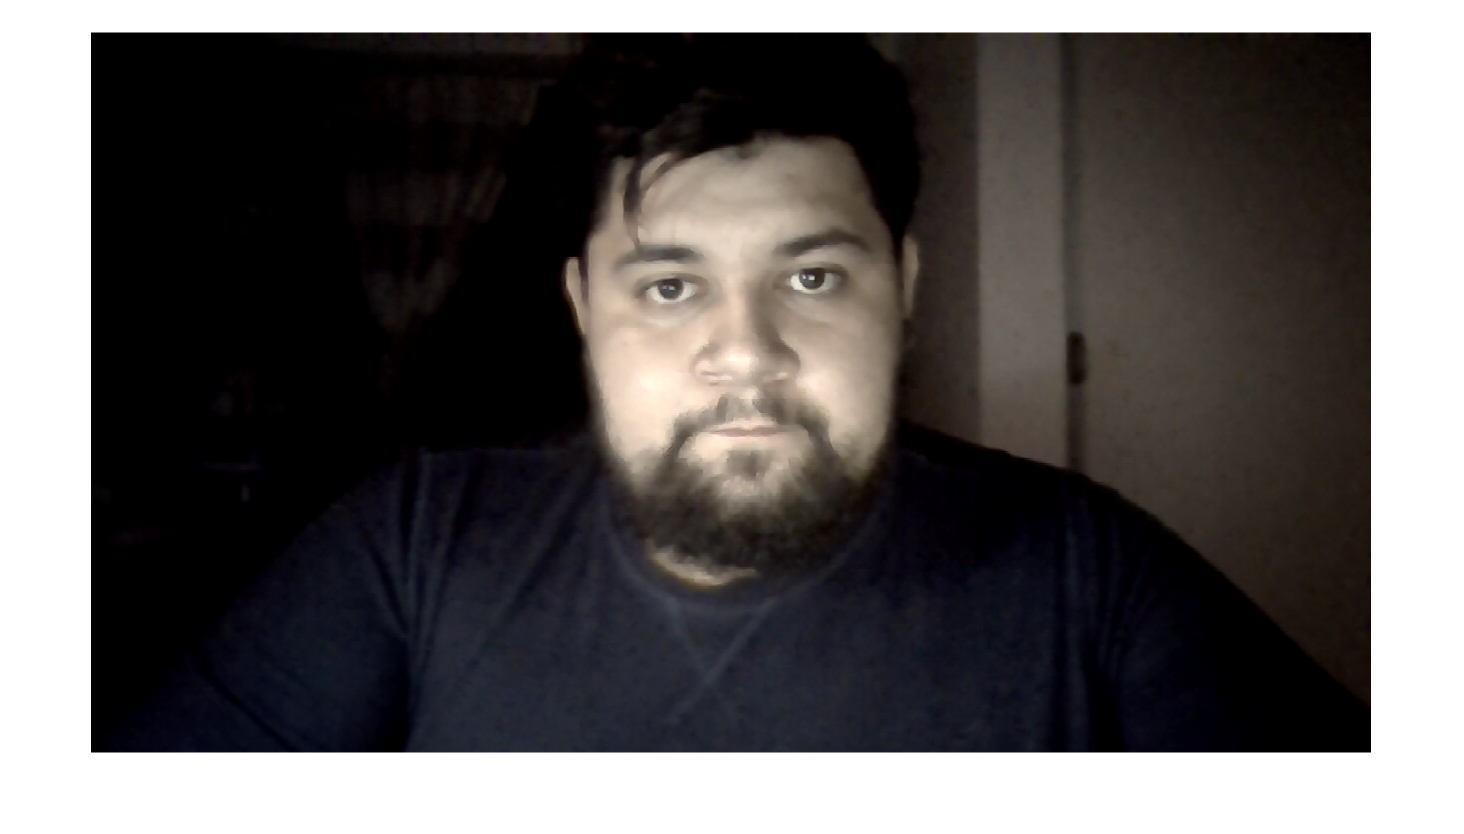
\includegraphics[width=\textwidth]{img1.png}
	\end{figure*}
	
	\begin{figure*}[!]
		\centering
		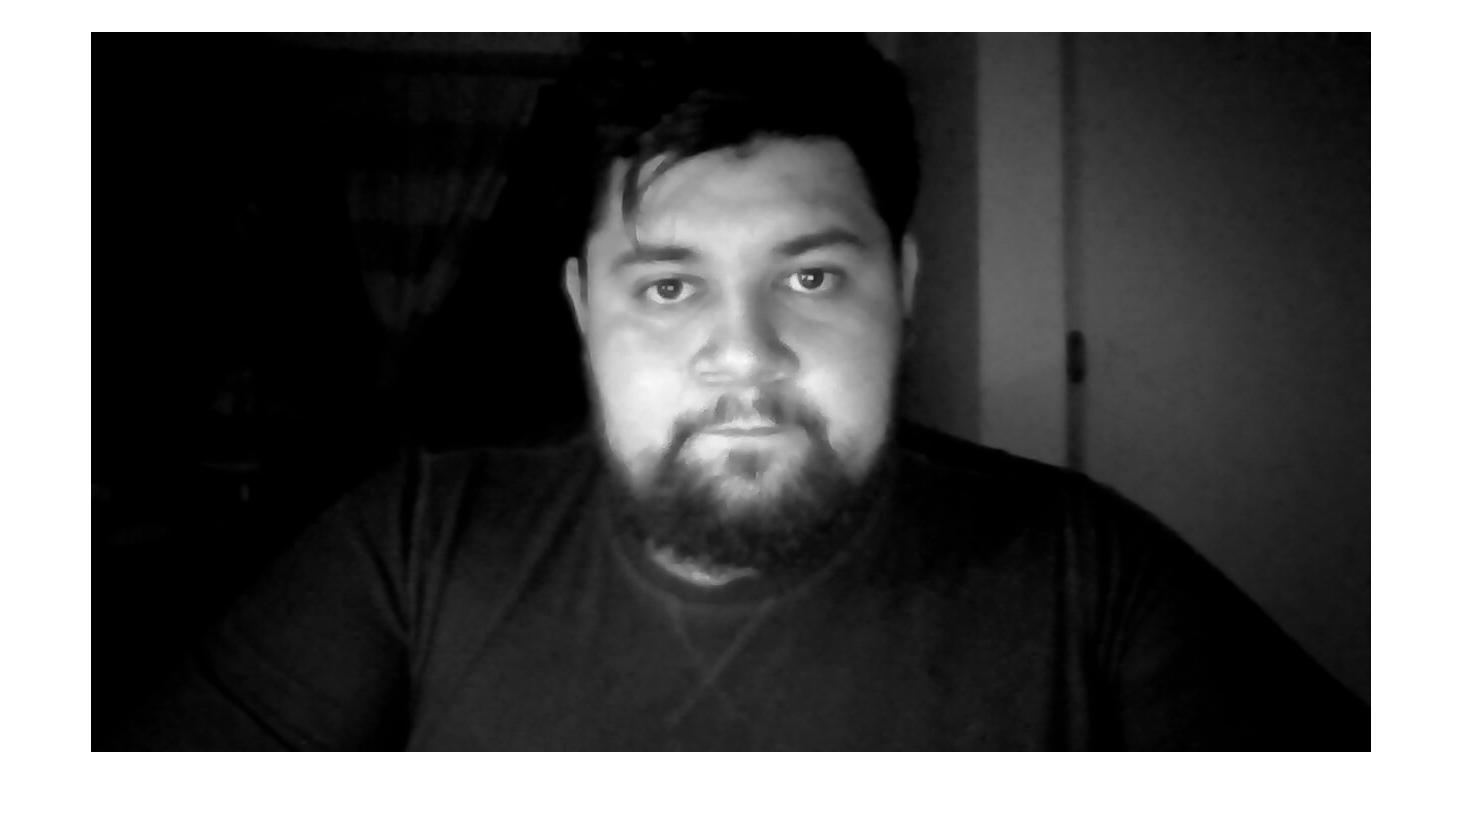
\includegraphics[width=\textwidth]{img2.png}
	\end{figure*}
	
	
	\newpage
	
	\section{Conclusión}
	
	En resumen, esta práctica nos ha permitido adquirir conocimientos y habilidades en la captura de imágenes mediante un periférico y el uso de la cámara de video. Hemos aprendido a interactuar con la cámara, capturar imágenes y procesarlas según nuestras necesidades, gracias a las herramientas proporcionadas por MATLAB. Estas habilidades son fundamentales en el ámbito científico y tecnológico actual, y nos brindan la capacidad de realizar investigaciones y desarrollos innovadores en diversas áreas.
	
\end{document}